\documentclass{article}
\usepackage{fancyhdr}
\usepackage{amsthm}
\usepackage{amssymb}
\usepackage{etoolbox}
\usepackage{verbatim}
\usepackage{enumerate}
\usepackage{amsmath}
\usepackage{algorithmicx}
\usepackage{algorithm}
\usepackage{algpseudocode}
\usepackage{tikz}
\usepackage{graphicx}

	
\pagestyle{fancy}
\title{Chapter 4}
\author{Michelle Bodnar, Andrew Lohr}

\newcounter{curnum}
\setcounter{curnum}{0}

\newtheorem{th1}{Exercise} 
\newcommand{\calH}{\mathcal{H}}
\newcommand{\calX}{\mathcal{X}}
\newcommand{\calA}{\mathcal{A}}
\newcommand{\calY}{\mathcal{Y}}

\begin{document}
\maketitle

\noindent\textbf{Exercise 4.1-1}\\

It will return the least negative position. As each of the cross sums are computed, the most positive one must have the shorest possible lengths. The algoritm doesn't consider length zero sub arrays, so it must have length 1.\\

\noindent\textbf{Exercise 4.1-2}\\

\begin{algorithm}
\caption{Brute Force Algorithm to Solve Maximum Subarray Problem}
\begin{algorithmic}
\State $left = 1$
\State $right = 1$
\State $max = A[1]$
\State $curSum = 0$
\For{$i=1$ to $n$} // Increment left end of subarray
	\State $curSum = 0$
	\For{$j=i$ to $n$} // Increment right end of subarray
		\State $curSum = curSum + A[j]$
		\If{$curSum > max$}
			\State $max = curSum$
			\State $left = i$
			\State $right = j$
		\EndIf
	\EndFor
\EndFor
\end{algorithmic}
\end{algorithm}

\noindent\textbf{Exercise 4.1-3}\\
The crossover point is at around a length 20 array, however, the times were incredibly noisy and I think that there was a garbage collection during the run, so it is not reliable. It would probably be more effective to use an acutal profiler for measuring runtimes. By switching over the way the recursive algorithm handles the base case, the recursive algorithm is now better for smaller values of $n$. The chart included has really strange runtimes for the brute force algorithm. These times were obtained on a Core 2 duo P8700 and java 1.8.0.51.

In the chart of runtimes, the x axis is the length of the array input. The y axis is the measured runtime in nanoseconds.\\

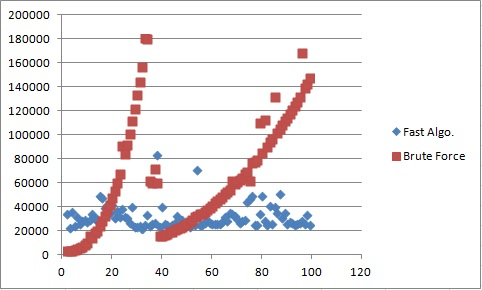
\includegraphics{4(1)}


\noindent\textbf{Exercise 4.1-4}\\

First do a linear scan of the input array to see if it contains any positive entries.  If it does, run the algorithm as usual.  Otherwise, return the empty subarray with sum 0 and terminate the algorithm. \\

\noindent\textbf{Exercise 4.1-5}\\

See the algorithm labeled linear time maximum subarray.

\begin{algorithm}
\caption{linear time maximum subarray(A)}
\begin{algorithmic}[1]
\State $M =-\infty$
\State $low_M, high_M = null$
\State $M_r = 0$
\State $low_r = 1$
\For{$i$ from 1 to A.length}
\State $M_r += A[i]$
\If {$M_r>M$}
\State $low_M = low_r$
\State $high_M = i$
\State $M= M_r$
\EndIf
\If {$M_r <0$}
\State $M_r = 0$
\State $low_r = i+1$
\EndIf
\State \Return $(low_M,high_M,M)$
\EndFor


\end{algorithmic}
\end{algorithm}

\noindent\textbf{Exercise 4.2-1}\\

\begin{align*}
S_1 &= 8-2=6\\
S_2 &= 1+3 = 4\\
S_3 &=7+5 = 12\\
S_4 &=4-6 = -2\\
S_5 &=1+5=6\\
S_6 &=6+2=8\\
S_7 &=3-5=-2\\
S_8 &=4 +2=6\\
S_9 &=1-7 = -6\\
S_{10} &=6+8=14
\end{align*}
\begin{align*}
P_1 &=6\\
P_2 &=8\\
P_3 &=72\\
P_4 &=-10\\
P_5 &=48\\
P_6 &=-12\\
P_7 &=-84
\end{align*}
\begin{align*}
C_{11} &=48 -10-8-12 = 18\\
C_{12} &= 6+8 = 14\\
C_{21} &= 72-10 = 62\\
C_{22} &=48+6-72+84 = 66
\end{align*}
So, we get the final result:

\[
\left(\begin{array}{c c}18&14\\62&66\end{array}\right)
\]\\

\noindent\textbf{Exercise 4.2-2}\\

As usual, we will assume that $n$ is an exact power of 2 and $A$ and $B$ are $n$ by $n$ matrices.  Let $A[i..j][k..m]$ denote the submatrix of $A$ consisting of rows $i$ through $j$ and columns $k$ through $m$. \\
\begin{algorithm}
\caption{Strassen(A, B)}
\begin{algorithmic}
\If{$A.length == 1$}
	\State \Return $A[1]\cdot B[1]$
\EndIf
\State Let $C$ be a new $n$ by $n$ matrix
\State $A11 = A[1..n/2][1..n/2]$
\State $A12 = A[1..n/2][n/2+1..n]$
\State $A21 = A[n/2+1..n][1..n/2]$
\State $A22 = A[n/2+1..n][n/2+1..n]$
\State $B11 = B[1..n/2][1..n/2]$
\State $B12 = B[1..n/2][n/2+1..n]$
\State $B21 = B[n/2+1..n][1..n/2]$
\State $B22 = B[n/2+1..n][n/2+1..n]$
\State $S_1 = B12-B22$
\State $S_2 = A11+A12$
\State $S_3 = A21 + A22$
\State $S_4 = B21-B11$
\State $S_5 = A11 + A22$
\State $S_6 = B11 + B22$
\State $S_7 = A12 - A22$
\State $S_8 = B21 + B22$
\State $S_9 = A11 - A21$
\State $S_{10} = B11 + B12$
\State $P_1 = Strassen(A11, S_1)$
\State $P_2 = Strassen(S_2, B22)$
\State $P_3 = Strassen(S_3, B11)$
\State $P_4 = Strassen(A22, S_4)$
\State $P_5 = Strassen(S_5, S_6)$
\State $P_6 = Strassen(S_7, S_8)$
\State $P_7 = Strassen(S_9, S_{10})$
\State $C[1..n/2][1..n/2] = P_5 + P_4 - P_2 + P_6$
\State $C[1..n/2][n/2+1..n] = P_1 + P_2$
\State $C[n/2+1..n][1..n/2] = P_3 + P_4$
\State $C[n/2+1..n][n/2+1..n] = P_5 + P_1 - P_3 - P_7$ 
\State \Return $C$
\end{algorithmic}
\end{algorithm}


\noindent\textbf{Exercise 4.2-3}\\

you could pad out the input matrices to be powers of two and then run the given algorithm. Padding out the the next largest power of two (call it $m$) will at most double the value of n because each power of two is off from wach other by a factor of two. So, this will have runtime
\[
m^{\lg 7} \le (2n)^{\lg 7} = 7 n^{\lg 7} \in O(n^{\lg 7})
\]
and
\[
m^{\lg 7} \ge n^{\lg 7} \in \Omega(n^{\lg 7})
\]
Putting these together, we get the runtime is $\Theta(n^{\lg 7})$.\\

\noindent\textbf{Exercise 4.2-4}\\

Assume that $n = 3^m$ for some $m$.  Then, using block matrix multiplication, we obtain the recursive running time $T(n) = kT(n/3) + O(1)$.  Using the Master theorem, we need the largest integer $k$ such that $\log_3 k < \lg 7$.  This is given by $k=21$.\\

\noindent\textbf{Exercise 4.2-5}\\

If we take the three algorithms and divide the number of multiplications by the side length of the matrices raised to $\lg(7)$, we approximately get the following values
\begin{align*}
&3745\\
&3963\\
&4167\\
\end{align*}
This means that, if used as base cases for a Strassen Algorithm, the first one will perform best for very large matrices.\\

\noindent\textbf{Exercise 4.2-6}\\

By considering block matrix multiplication and using Strassen's algorithm as a subroutine, we can multiply a $kn \times n$ matrix by an $n \times kn$ matrix in $\Theta(k^2n^{\log 7})$ time.  With the order reversed, we can do it in $\Theta(k n^{\log 7})$ time. \\

\noindent\textbf{Exercise 4.2-7}\\

We can see that the final result should be
\[
(a+bi)(c+di) = ac-bd +(cb+ad) i
\]

We will be multiplying 
\begin{align*}
P_1 &= (a+b)c = ac+bc
P_2 &= b(c+d) = bc+bd
P_3&= (a-b)d = ad+bd
\end{align*}

Then, we can recover the real part by taking $P_1 - P_2$ and the imaginary part by taking $P_2+P_3$.\\

\noindent\textbf{Exercise 4.3-1}\\

Inductively assume $T(n)\le c n^2$, were $c$ is taken to be $\max(1,T(1))$ then
\[
T(n) = T(n-1)+n \le c(n-1)^2 +n = c n^2 +(1-2c)n + 1 \le c n^2 +2-2c \le c n^2
\]
The first inequality comes from the inductive hypothesis, the second from the fact that $n\ge 1$ and $1-2c <0$. The last from the fact that $c\ge 1$.\\

\noindent\textbf{Exercise 4.3-2}\\

We'll show $T(n) \leq 3 \log n - 1$, which will imply $T(n) = O(\log n)$.
\begin{align*}
T(n) &= T(\lceil n/2 \rceil) + 1 \\
&\leq 3\log(\lceil n/2 \rceil) - 1 + 1 \\
&\leq 3\log(3n/4) \\
&= 3 \log n + 3 \log(3/4) \\
&\leq 3 \log n  + \log(1/2) \\
& = 3 \log n - 1. 
\end{align*}

\noindent\textbf{Exercise 4.3-3}\\

Inductively assume that $T(n) \le cn\lg n$ where $c = \max(T(2)/2,1)$. Then, 
\[
T(n) = 2 T(\lfloor n/2\rfloor) + n \le 2 c\lfloor n/2 \rfloor \lg(\lfloor n/2\rfloor) +n
\]
\[
\le cn \lg(n/2) +n = cn (\lg(n) - 1) +n = cn(\lg(n) -1+\frac{1}{c}) \le cn\lg(n)
\]
And so, $T(n)\in O(n\lg(n))$.

Now, inductively assume that $T(n)\ge c'n\lg(n)$ where $c' = \min(1/3, T(2)/2)$. 
\[
T(n) = 2 T(\lfloor n/2 \rfloor) +n \ge 2c'\lfloor n/2 \rfloor \lg(\lfloor n/2 \rfloor) + n \ge c'(n-1) \lg((n-1)/2) +n
\]
\[
= c'(n-1)(\lg(n) - 1 - \lg(n/(n-1))) +n\]\[ = c' n (\lg(n) -1 -\lg(n/(n-1)) + \frac{1}{c'}) - c'(\lg(n) - 1 -\lg(n/(n-1)))
\]
\[
\ge c'n(\lg(n)-2 + \frac{1}{c'} - \frac{(\lg(n-1) - 1 )}{n}) \ge c'n(\lg(n)-3 + \frac{1}{c'}) \ge c'n\lg(n)
\]
So, $T(n)\in \Omega(n)$. Together with the first part of this problem, we get that $T(n)\in \Theta(n)$.\\

\noindent\textbf{Exercise 4.3-4}\\

We'll use the induction hypothesis $T(n) \leq 2n \log n + 1$. First observe that this means $T(1) = 1$, so the base case is satisfied.  Then we have
\begin{align*}
T(n) &= 2T(\lfloor n/2 \rfloor) + n\\
&\leq 2((2n/2)\log(n/2) + 1) + n \\
&= 2n\log(n) - 2n \log 2 + 2 + n \\
&= 2n \log(n) + 1 + n + 1 - 2n \\
& \leq 2n \log(n) + 1.
\end{align*}

\noindent\textbf{Exercise 4.3-5}\\

Will be done later\\

\noindent\textbf{Exercise 4.3-6}\\

Choose $n_1$ such that $n \geq n_1$ implies $n/2 + 17 \leq 3n/4$.  We'll find $c$ and $d$ such that $T(n) \leq cn\log n - d$.
\begin{align*}
T(n) &= 2T(\lfloor n/2 \rfloor + 17) + n \\
&\leq 2(c(n/2 + 17)\log(n/2 + 17) - d) + n \\
&\leq cn\log(n/2 + 17) + 17c\log(n/2 + 17) - 2d + n \\
&\leq cn\log(3n/4) + 17c\log(3n/4) - 2d + n\\
&= cn\log n - d +cn\log(3/4) + 17c\log(3n/4) - d + n.
\end{align*}

Take $c = -2/\log(3/4)$ and $d =34$.  Then we have $T(n) \leq cn\log n - d + 17c\log(n) - n$.  Since $\log(n) = o(n)$, there exists $n_2$ such that $n \geq n_2$ implies $n \geq 17c\log(n)$.  Letting $n_0 = \max\{n_1, n_2\}$ we have that $n \geq n_0$ implies $T(n) \leq cn\log n - d$.  Therefore $T(n) = O(n \log n)$. \\

\noindent\textbf{Exercise 4.3-7}\\

We first try the substitution proof $T(n) \le cn^{\log_34}$.
\[
T(n) = 4T(n/3)+n \le 4 c(n/3)^{\log_34}+n = 4cn^{\log_34}+n
\]
This clearly will not be $\le cn^{\log_34}$ as required.

Now, suppose instead that we make our inductive hypothesis $T(n) \le cn^{\log_34} -3n$.
\[
T(n) = 4T(n/3)+n \le 4(c(n/3)^{\log_34}-n) +n = cn^{\log_34} - 4n + n =cn^{\log_34} - 3n 
\]
as desired.\\


\noindent\textbf{Exercise 4.3-8} \\

Suppose we want to use substitution to show $T(n) \leq cn^2$ for some $c$.  Then we have
\begin{align*}
T(n) &= 4T(n/2) + n \\
&\leq 4(c(n/2)^2) + n \\
&= cn^2 + n,
\end{align*}
which fails to be less than $cn^2$ for any $c > 0$.  Next we'll attempt to show $T(n) \leq cn^2 - n$.
\begin{align*}
T(n)&= 4T(n/2) + n\\
& \leq 4(c(n/2)^2 - n) + n \\
&= cn^2 - 4cn + n \\
&\leq cn^2 
\end{align*}
provided that $c \geq 1/4$.  \\

\noindent\textbf{Exercise 4.3-9}\\

Consider $n$ of the form $2^k$. Then, the recurrence becomes
\[
T(2^k) = 3 T(2^(k/2)) +k
\]
We define $S(k) = T(2^k)$. So,
\[
S(k) =3S(k/2)+k
\]
We use the inductive hypothesis $S(k)\le (S(1)+2) k^{\log_23} - 2k$
\[
S(k) = 3S(k/2)+k \le 3(S(1)+2)(k/2)^{\log_23} -3k+k = (S(1)+2)k^{\log_23} - 2k
\]
as desired. Similarly, we show that $S(k) \ge (S(1)+2) k^{\log_23} -2k$
\[
S(k) = 3S(k/2) +k \ge (S(1)+2)k^{\log_23} -2k
\]
So, we have that $S(k) = (S(1)+2)k^{\log_23}-2k$. Translating this back to $T$, $T(2^k) = (T(2)+2) k^{\log_23} -2k$. So, $T(n) = (T(2)+2)(\lg(n))^{\log_23} - 2\lg(n)$.\\

\noindent\textbf{Exercise 4.4-2}\\

As we construct the tree, there is only one node at depth $d$, and its weight is $n^2/(2^d)^2$.  Since the tree has $\log(n)$ levels, we guess that the solution is roughly $\sum_{i=0}^{\log n} \frac{n^2}{4^i} = O(n^2)$.  Next we use the substitution method to verify that $T(n) \leq cn^2$.  
\begin{align*}
T(n) &= T(n/2) + n^2 \\
& \leq c(n/2)^2 + n^2 \\
& = (\frac{c}{4} + 1)n^2 \\
&\leq cn^2
\end{align*}
provided that $c \geq 4/3$.  \\

\noindent\textbf{Exercise 4.4-4}\\

The recursion tree looks like a complete binary tree of height $n$ with cost 1 at each node.  Thus we guess that the solution is $O(2^n)$.  We'll use the substitution method to verify that $T(n) \leq 2^n - 1$. 
\begin{align*}
T(n) &= 2T(n-1) + 1 \\
&\leq 2(2^{n-1} - 1) + 1 \\
&= 2^n - 1.
\end{align*}

\noindent\textbf{Exercise 4.4-6}\\

Examining the tree in figure 4.6 we observe that the cost at each level of the tree is exactly $cn$.  To find a lower bound on the cost of the algorithm, we need a lower bound on the height of the tree.  The shortest simple path from root to leaf is found by following the left child at each node.  Since we divide by 3 at each step, we see that this path has length $\log_3 n$, so the cost of the algorithm is $cn(\log_3 n + 1) \geq cn\log_3 n = \frac{c}{log 3} n \log n = \Omega(n \log n)$. \\

\noindent\textbf{Exercise 4.4-8}\\

\begin{tikzpicture}
\path (0,10) node (a) {$T(a) + cn$}
(0,8) node (b) {$T(a) + c(n-a)$}
(0,6) node (c) {$T(a) + c(n-2a)$}
(0,4) node (d) {$T(1)$};

\draw (0,9.5) -- (0,8.5);
\draw (0,6.5) -- (0,7.5);
\draw[dashed] (0,4.5) -- (0,5.5);
\end{tikzpicture}

Since each node of the recursion tree has only one child, the cost at each level is just the cost of the node.  Moreover, there are $\lceil n/a \rceil$ levels in the tree.  Summing the cost at each level we see that the total cost of the algorithm is 
\[ \sum_{i=0}^{\lceil n/a \rceil - 1} T(a) + c(n-ia) = \lceil n/a \rceil T(a) + c\lceil n/a \rceil n - ca \frac{\lceil n/a \rceil(\lceil n/a \rceil - 1)}{2}.\]

To compute the asymptotoics we can assume $n$ is divisible by $a$ and ignore the ceiling functions.  Then this becomes
\[ \frac{c}{2a}n^2 + (T(a)/a + c/2)n = \Theta(n^2).\]\\


\noindent\textbf{Exercise 4.5-1}\\

\begin{enumerate}[a)]
\item
$\Theta(\sqrt{n})$
\item
$\Theta(\sqrt{n}\lg(n))$
\item
$\Theta(n)$
\item
$\Theta(n^2)$
\end{enumerate}

\noindent\textbf{Exercise 4.5-2}\\

Recall that Strassen's algorithm has running time $\Theta(n^{\lg 7})$.  We'll choose $a = 48$.  This is the largest integer such that $\log_4(a) < \lg 7$.  Moreover, $2 < \log_4(48)$ so there exists $\epsilon > 0$ such that $n^2 < n^{\log_4(48) - \epsilon}$.  By case 1 of the Master theorem, $T(n) = \Theta(n^{\log_4(48)})$ which is asymptotically better than $\Theta(n^{\lg 7})$. \\

\noindent\textbf{Exercise 4.5-3}\\

Applying the method with $a=1,b=2$, we have that $\Theta(n^{\log_1 2}) = \Theta(1)$. So, we are in the second case, so, we have a final result of $\Theta(n^{\log_1 2}\lg(n)) = \Theta(\lg(n))$.\\

\noindent\textbf{Exercise 4.5-4}\\

The master method cannot be applied here.  Observe that $\log_b a = \log_2 4 = 2$ and $f(n) = n^2 \lg n$.  It is clear that cases 1 and 2 do not apply.  Furthermore, although $f$ is asymptotically larger than $n^2$, it is not polynomially larger, so case 3 does not apply either.  We'll show $T(n) = O(n^2\lg^2 n)$.  To do this, we'll prove inductively that $T(n) \leq n^2\lg^2 n$.  
\begin{align*}
T(n) & = 4T(n/2)+n^2\lg n \\
& \leq 4((n/2)^2\lg^2(n/2)) + n^2 \lg n \\
&= n^2(\lg n - \lg 2)^2 + n^2 \lg n \\
&= n^2\lg^2 n - n^2(2\lg n - 1 - \lg n) \\
&= n^2\lg^2 n - n^2(\lg n - 1) \\
&\leq n^2\lg^2 n
\end{align*}
provided that $n \geq 2$.  \\

\noindent\textbf{Exercise 4.5-5}\\

Let $\epsilon = a=1,b=3$, and $f = 3n + 2^{3n} \chi_{\{2^i:i\in\mathbb{N}\}}$ where $\chi_A$ is the indicator function of the set $A$. Then, we have that for any number $n$ which is three times a power of 2, we know that 
\[
f(n) = 3n < 2^n + n = f(n/3)
\]
And so, it fails the regularity condition, even though $f \in \Omega(n) =\Omega(n^{\log_b(a) + \epsilon})$.\\


\noindent\textbf{Exercise 4.6-1}\\

$n_j$ is obtained by shifting the base $b$ representation $j$ positions to the right, and adding 1 if any of the $j$ least significant positions are non-zero.\\

\noindent\textbf{Exercise 4.6-2}\\

Assume that $n = b^m$ for some $m$.  Let $c_1$ and $c_2$ be such that $c_2n^{\log_b a}\lg^k n \leq f(n) \leq c_1 n^{\log_b a}\lg^k n$.  We'll first prove by strong induction that $T(n) \leq n^{\log_b a}\lg^{k+1}n - d n^{\log_b a}\lg^k n$ for some choice of $d \geq 0$.  Equivalently, that $T(b^m) \leq a^m \ln^{k+1}(b^m) - da^m\lg^k(b^m)$.  
\begin{align*}
T(b^m) &= aT(b^m/b) + f(b^m) \\
&\leq a(a^{m-1} \lg^{k+1}(b^{m-1}) - da^{m-1}\lg^k b^{m-1}) + c_1 a^m\lg^k (b^m) \\
&= \leq a^m \lg^{k+1}(b^{m-1}) - da^m\lg^k b^{m-1} + c_1 a^m\lg^k (b^m) \\
&= \leq a^m [\lg(b^m) - \lg b]^{k+1} -  da^m[\lg b^m - \lg b]^k + c_1 a^m\lg^k (b^m)\\
&= a^m\lg^{k+1}(b^m) -  da^md\lg^k b^m -a^m \left(d \sum_{r=0}^{k-1}{k \choose r}\lg^r(b^m)(-\lg b)^{k-r} + \sum_{r = 0}^k {k+1 \choose r} \lg^r(b^m)(-\lg(b))^{k+1-r}  + c_1 \lg^k (b^m)\right) \\
&=  a^m\lg^{k+1}(b^m) -  da^m\lg^k b^m - a^m\left((c_1 - k\lg b)\lg^k(b^m) + \sum_{r = 0}^{k-1} {k+1 \choose r} \lg^r(b^m)(-\lg(b))^{k+1-r} + d \sum_{r=0}^{k-1}{k \choose r}\lg^r(b^m)(-\lg b)^{k-r}\right) \\
& \leq a^m\lg^{k+1}(b^m) -  da^m\lg^k b^m
\end{align*}
for $c_1 \geq k \lg b$.  Thus $T(n) = O(n^{\log_b a}\lg^{k+1}n)$.  A similar analysis shows $T(n) = \Omega(n^{\log_b a}\lg^{k+1}n)$.\\

\noindent\textbf{Exercise 4.6-3}\\

Suppose that $f$ satisfies the regularity condition, we want that $\exists \epsilon, d,k$,$\forall n\ge k$, we have $f(n) \ge d n^{\log_b a +\epsilon}$. By the regularity condition, we have that for sufficiently large $n$, $af(n/b) \le cf(n)$. In particular, it is true for all $n\ge bk$. Let this be our $k$ from above, also, $\epsilon= -\log_b(c)$. Finally let $d$ be the largest value of $f(n)/n^{\log_b(a)+\epsilon}$ between $bk$ and $b^2k$. Then, we will prove by induction on the highest $i$ so that $b^i k$ is less than $n$ that for every $n\ge k, f(n) \ge d n^{\log_b a +\epsilon}$. By our definition of $d$, we have it is true for $i= 1$. So, suppose we have $b^{i-1}k < n \le b^i k$. Then, by regularity and the inductive hypothesis,  $cf(n) \ge a f(n/b) \ge ad \left(\frac{n}{b}\right)^{\log_b(a) +\epsilon}$. Solving for $f(n)$, we have
\[
f(n) \ge \frac{ad}{c} \left(\frac{n}{b}\right)^{\log_b{a/c}} = \frac{a/c}{b^{\log_b(a/c)}} d n^{\log_b(a) + \epsilon} =  d n^{\log_b(a) + \epsilon}
\]
Completing the induction. \\



\noindent\textbf{Problem 4-1}\\

\begin{enumerate}[a)]
\item
By Master Theorem, $T(n) \in \Theta(n^4)$

\item
By Master Theorem, $T(n) \in \Theta(n)$

\item
By Master Theorem, $T(n) \in \Theta(n^2\lg(n))$

\item
By Master Theorem, $T(n) \in \Theta(n^2)$

\item
By Master Theorem, $T(n) \in \Theta(n^{\lg(7)})$

\item
By Master Theorem, $T(n) \in \Theta(n^{1/2}\lg(n))$

\item
Let $d = m\mod 2$, we can easily see that the exact value of $T(n)$ is
\[
\sum_{j=1}^{j=n/2} (2j+d)^2 = \sum_{j=1}^{n/2}4j^2 + 4jd + d^2 = \frac{n(n+2)(n+1)}{6} + \frac{n(n+2)d}{2} + \frac{d^2n}{2}
\]
This has a leading term of $n^3/6$, and so $T(n) \in \Theta(n^3)$

\end{enumerate}

\noindent\textbf{Problem 4-2}\\

a. \\

1. $T(n) = T(n/2) + \Theta(1)$.  Solving the recursion we have $T(N) = \Theta(\lg N)$.

2. $T(n) = T(n/2) + \Theta(N)$.  Solving the recursion we have $T(N) = \Theta(N \lg N)$.

3. $T(n) = T(n/2) + \Theta(n/2)$. Solving the recursion we have $T(N) = \Theta(N)$. \\

b.\\

  1. $T(n) = 2T(n/2) + cn$. Solving the recursion we have $T(N) = \Theta(N\lg N)$.

2. $T(n) = 2T(n/2) + cn + 2\Theta(N)$.  Solving the recursion we have $T(N) = \Theta(N\lg N) + \Theta(N^2) = \Theta(N^2)$.

3. $T(n) = 2T(n/2) + cn + 2c'n/2$.  Solving the recursion we have $T(N) = \Theta(N\ln N)$. \\

\noindent\textbf{Problem 4-3}\\

\begin{enumerate}[a)]
\item
By Master Theorem, $T(n) \in \Theta(n^{\log_3(4)})$

\item
We first show by substitution that $T(n)\le n\lg(n)$.

\[
T(n) = 3T(n/3) + n/\lg(n) \le cn\lg(n) - cn\lg(3) + n/\lg(n) = cn\lg(n) + n(\frac{1}{\lg(n)} - c \lg(3)) \le cn\lg(n)
\]

now, we show that $T(n) \ge cn^{1-\epsilon}$ for every $\epsilon>0$.

\[
T(n) = 3T(n/3) + n/\lg(n) \ge 3 c/3^{1-\epsilon}n^{1-\epsilon} + n/\lg(n) = 3^{\epsilon}cn^{1-\epsilon} +n/\lg(n)
\]
showing that this is $\le cn^{1-\epsilon}$ is the same as showing
\[
3^{\epsilon} + n^{\epsilon}/(c\lg(n)) \ge 1
\]
Since $\lg(n)\in o(n^{\epsilon})$ this inequality holds. So, we have that The function is soft Theta of $n$, see problem 3-5.

\item
By Master Theorem, $T(n) \in \Theta(n^{2.5})$


\item
it is $\Theta(n\lg(n))$. The subtraction occurring inside the argument to $T$ won't change the saymptotics of the solution, that is, for large $n$ the division is so much more of a change than the subtraction that it is the only part that matters. once we drop that subtraction, the solution comes by the master theorem.% To see this, we can write $S(n) = T(\lg(n))$, then, $S(n) = T(\lg(n)) = 3T(\lg(\sqrt[3]{n}/2^3)) + \lg(n) = 3S(\sqrt[3]{n}/8) + \lg(n)$

\item
By the same reasoning as part 2, the function is $O(n\lg(n))$ and $\Omega(n^{1-\epsilon})$ for every $\epsilon$ and so is soft theta of $n$, see problem 3-5.

\item

We will show that this is $O(n)$ by substitution. We want that $T(k) \le ck$ for $k<n$, then, 
\[
T(n) = T(n/2) + T(n/4)+T(n/8) + n \le \frac{7}{8}cn + n 
\]

So, this is $\le cn$ so long as $\frac{7}{8}c +1 \le c$ which happens whenever $c\ge 8$.

\item
Recall that $\chi_A$ denotes the indicator function of $A$, then, we see that the sum is
\[
T(0) + \sum_{j=1}^{n} \frac{1}{j} = T(0) + \int_{1}^{n+1} \sum_{j=1}^{n+1} \frac{\chi_{(j,j+1)}(x)}{j} dx 
\]
However, since $\frac{1}{x}$ is monatonically decreasing, we have that for every $i\in \mathbb{Z}^+$,
\[
\sup_{x\in (i,i+1)}  \sum_{j=1}^{n+1} \frac{\chi_{(j,j+1)}(x)}{j}  - \frac{1}{x} = \frac{1}{i}  - \frac{1}{i+1} = \frac{1}{i(i+1)}
\]
So, our expression for $T(n)$ becomes
\[
T(N) = T(0)+ \int_1^{n+1} \left(\frac{1}{x} + O(\frac{1}{\lfloor x\rfloor(\lfloor x\rfloor+1)}\right)dx
\]
We deal with the error term by first chopping out the constant amount between 1 and 2 and then bound the error term by $O(\frac{1}{x(x-1)})$ which has an antiderivative (by method of partial fractions) that is $O(\frac{1}{n})$. so,

\[
T(N) = \int_1^{n+1} \frac{dx}{x} + O(\frac{1}{n} = \lg(n) + T(0) + \frac{1}{2} + O(\frac{1}{n})
\]
This gets us our final answer of $T(n) \in \Theta(\lg(n))$
\item
we see that we explicity have
\[
T(n) = T(0) +\sum_{j=1}^n \lg(j) = T(0) + \int_1^{n+1} \sum_{j=1}^{n+1} \chi_{(j,j+1)}(x)\lg(j) dx 
\]
Similarly to above, we will relate this sum to the integral of $\lg(x)$. 
\[
\sup_{x\in (i,i+1)}  \left|\sum_{j=1}^{n+1} \chi_{(j,j+1)}(x)\lg(j)  - \lg(x)\right| = \lg(j+1) - \lg(j) = \lg\left(\frac{j+1}{j}\right)
\]
So, 
\[
T(n) \le \int_{i}^n \lg(x+2) + \lg(x) - \lg(x+1) dx  = (1  + O(\frac{1}{\lg(n)}))\Theta(n\lg(n))
\]
\item
See the approach used in the previous two parts, we will get $T(n) \in \Theta(li(n))= \Theta( \frac{n}{\lg(n)})$
\item
Let $i$ be the smallest $i$ so that $n^{\frac{1}{2^i}}<2$. We recall from a previous problem (3-6.e) that this is $\lg(\lg(n))$ Expanding the recurrence, we have that it is 
\[
T(n) = n^{1 - \frac{1}{2^i}} T(2) + n + n \sum_{j=1}^i 1 \in \Theta(n\lg(\lg(n)))
\]

\end{enumerate}

\noindent\textbf{Problem 4-4}\\

a. Recall that $F_0 = 0$, $F_1 = 1$, and $F_i = F_{i-1} + F_{i-2}$ for $i \geq 2$.  Then we have
\begin{align*}
\mathcal{F}(z) &= \sum_{i=0}^\infty F_i z^i \\
&= F_0 + F_1z + \sum_{i=2}^\infty (F_{i-1} + F_{i-2})z^i \\
&= z + z\sum_{i=2}^\infty F_{i-1}z^{i-1} + z^2\sum_{i=2}^\infty F_{i-2}z^{i-2} \\
&= z + z\sum_{i=1}^\infty F_{i}z^{i} + z^2\sum_{i=0}^\infty F_{i}z^{i} \\
&= z + z\mathcal{F}(z) + z^2\mathcal{F}(z).
\end{align*}

b. Manipulating the equation given in part (a) we have $\mathcal{F}(z) - z\mathcal{F}(z) - z^2\mathcal{F}(z) = z$, so factoring and dividing gives 
\[ \mathcal{F}(z) = \frac{z}{1-z-z^2}.\]
Factoring the denominator with the quadratic formula shows $1 - z - z^2 = (1-\phi z)(1 - \hat{\phi} z)$, and the final equality comes from a partial fraction decomposition. \\

c. From part (b) and our knowledge of geometric series we have
\begin{align*}
 \mathcal{F}(z) &= \frac{1}{\sqrt{5}}\left(\frac{1}{1-\phi z} - \frac{1}{1-\hat{\phi}z}\right) \\
&= \frac{1}{\sqrt{5}}\left(\sum_{i=0}^\infty (\phi z)^i - \sum_{i=0}^\infty (\hat{\phi}z)^i \right) \\
&=\sum_{i=0}^\infty  \frac{1}{\sqrt{5}} (\phi^i - \hat{\phi}^i)z^i.
\end{align*}

d. From the definition of the generating function, $F_i$ is the coefficient of $z^i$ in $\mathcal{F}(z)$.  By part (c) this is given by $\frac{1}{\sqrt{5}} (\phi^i - \hat{\phi}^i)$. Since $|\hat{\phi}| < 1$ we must have $| \frac{\hat{\phi}^i}{\sqrt{5}} | < | \frac{\hat{\phi}}{\sqrt{5}} | < \frac{1}{2}$.  Finally, since the Fibonacci numbers are integers we see that the exact solution must be the approximated solution $\frac{\phi^i}{\sqrt{5}}$ rounded to the nearest integer. \\

\noindent\textbf{Problem 4-5}\\

\begin{enumerate}[a)]

\item
The strategy for the bad chips is to always say that other bad chips are good and other good chips are bad. This mirrors the strategy used by the good chips, and so, it would be impossible to distinguish

\item
Arbitrarily pair up the chips. Look only at the pairs for which both chips said the other was good. Since we have at least half of the chips being good, we know that there will be at least one such pair which claims the other is good. We also know that at least half of the pairs which claim both are good are actually good. Then, just arbirarily pick a chip from each pair and let these be the chips that make up the sub-instance of the problem

\item
Once we have indentified a single good chip, we can just use it to query every other chip. 
The recurrence from before for the number of tests to find a good chip was
\[
T(n) \le T(n/2) + n/2
\]
This has solution $\Theta(n)$ by the Master Theorem. So, we have the problem can be solved in $O(n)$ pairwise tests. Since we also neccesarily need to look at at least half of the chips, we know that the problem is also $\Omega(n)$.

\end{enumerate}

\noindent\textbf{Problem 4-6}\\

a. If an array $A$ is Monge then trivially it must satisfy the inequality by taking $k = i+1$ and $l = j+1$.  Now suppose $A[i,j] + A[i+1,j+1] \leq A[i,j+1] + A[i+1,j]$.  We'll use induction on rows and columns to show that the array is Monge.  The base cases are each covered by the given inequality.  Now fix $i$ and $j$, let $r \geq 1$, and suppose that $A[i,j] + A[i+1,j+r] \leq A[i,j+r] + A[i+1,j]$.  By applying the induction hypothesis and given inequality we have
\begin{align*}
A[i,j] + A[i+1,j+r+1] &\leq  A[i,j+r] + A[i+1,j] -  A[i+1,j+r] + A[i, j+r+1] + A[i+1, j+r] - A[i, j+r] \\
&=  A[i+1,j] + A[i, j+r+1]  \\
\end{align*}
so it follows that we can extend columns and preserve the Monge property.  Next we induct on rows.  Suppose that $A[i,j] + A[k,l] \leq A[i,l] + A[k,j]$.  Then we have
\begin{align*}
A[i,j] + A[k+1,l] &\leq A[i,l] + A[k,j] - A[k,l] +  A[k+1,l] \hspace{4.2cm} \mbox{by assumption} \\
&\leq  A[i,l] + A[k,j] - A[k,l] + A[k,l] + A[k+1,l-1] - A[k,l-1] \mbox{ by given inequality} \\
&=  A[i,l] + (A[k,j] + A[k+1,l-1]) - A[k,l-1] \\
&\leq A[i,l] + A[k,l-1] + A[k+1,j] - A[k,l-1] \hspace{3cm} \mbox{ by row proof} \\
&= A[i,l] + A[k+1,j].
\end{align*}

b. Change the 7 to a 5. \\

c. Suppose that there exist $i$ and $k$ such that $i < k$ but $f(i) > f(k)$.  Since $A$ is Monge we must have $A[i,f(k)] + A[k,f(i)] \leq A[k,f(k)] + A[i,f(i)]$. Since $f(i)$ gives the position of the leftmost minimum element in row $i$, this implies that $A[i,f(k)] > A[i,f(i)]$.  Moreover, $A[k, f(k)] \leq A[k,f(i)]$.  Combining these with the Monge inequality implies $A[i,f(i)] + A[k,f(i)] < A[k,f(i)] + A[i,f(i)]$, which is impossible since the two sides are equal.  Therefore no such $i$ and $k$ can exist. \\

d.  Linearly scan row 1 indices 1 through $f(2)$ for the minimum element of row 1 and record as $f(1)$.  Next linearly scan indices $f(2)$ through $f(4)$ of row 3 for the minimum element of row 3.  In general, we need only scan indices $f(2k)$ through $f(2k+2)$ of row $2k+1$ to find the leftmost minimum element of row $2k+1$.  If $m$ is odd, we'll need to search indices $f(m-1)$ through $n$ to find the leftmost minimum in row $m$.  By part (c) we know that the indices of the leftmost minimum elements are increasing, so we are guaranteed to find the desired minimum from among the indices scanned. An element of column $j$ will be scanned $N_j + 1$ times, where $N_j$ is the number of $i$ such that $f(i) = j$. Since $\sum_{j=1}^n N_j= n$, the total number of comparisons is $m + n$, giving a running time of $O(m+n)$. \\

e. Let $T(m,n)$ denote the running time of the algorithm applied to an $m$ by $n$ matrix.  $T(m,n) = T(m/2,n) + c(m+n)$ for some constant $c$.  We'll show $T(m,n) \leq c(m + n\log m) - 2cm$.
\begin{align*}
T(m,n) &= T(m/2,n) + c(m+n)\\
&\leq c(m/2 + n\log(m/2)) - 2cm + c(m+n) \\
&= c(m/2 + n\log m) - cn + cn - cm \\
& \leq c(m+n\log m) - cm
\end{align*}
so by induction we have $T(m,n) = O(m+n\log m)$.

\end{document}